
\begin{frame}{The basic problem}

%\adjincludegraphics[width=0.9\textwidth,trim={0 {.5\height} 0 0 }, clip]{static_figures/survey_and_voting.jpg}

We have a survey population, for whom we observe:
%
\begin{itemize}
 \item Covariates $\x$ (e.g.~race, gender, zip code, age, education level)
 \item Responses $\y$ (e.g.~A binary response to ``do you support policy such--and--such'')
\end{itemize}
%

We want the average response in a target population,
in which we observe only covariates.


\splitpage{
    \centering
    \only<1>{
    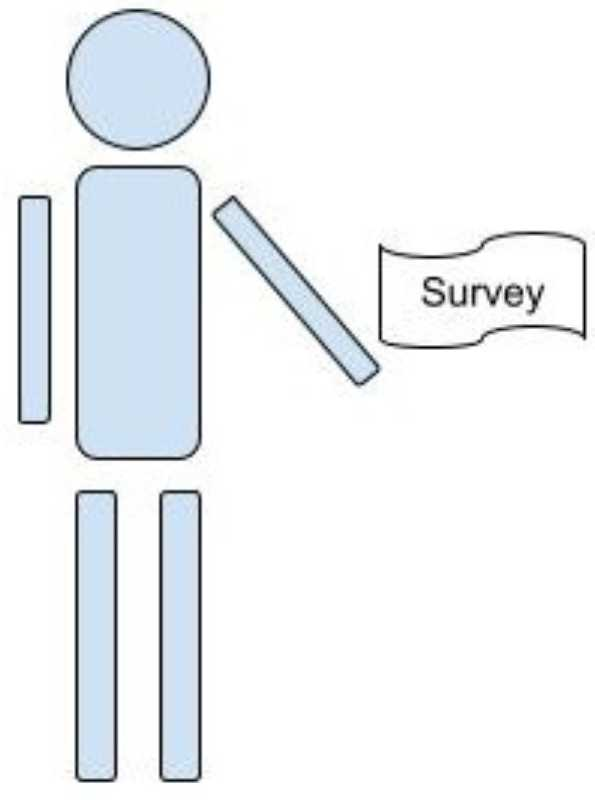
\includegraphics[width=0.5\textwidth]{static_figures/survey_man.jpg}
    }
    \only<2->{
    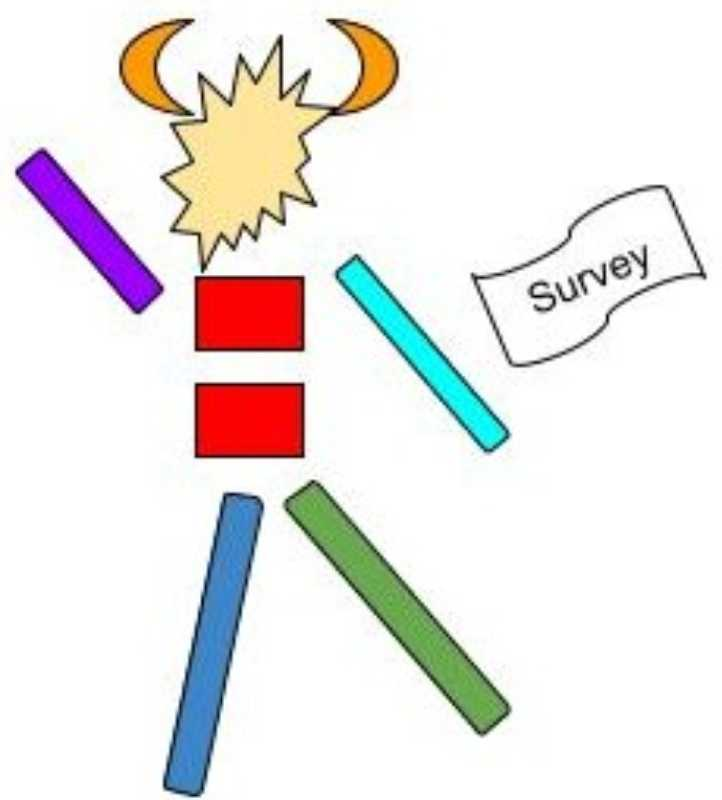
\includegraphics[width=0.5\textwidth]{static_figures/survey_crazy_man.jpg}
    }
}{
    \centering
    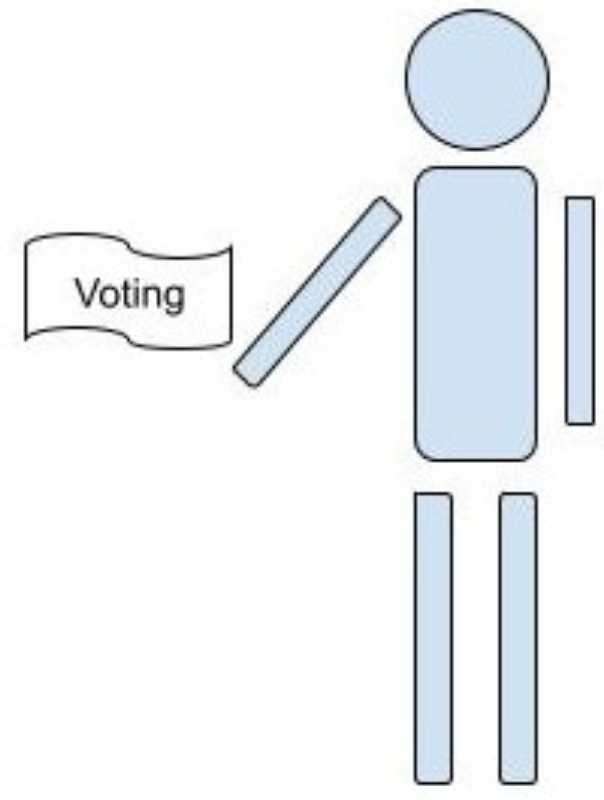
\includegraphics[width=0.5\textwidth]{static_figures/voting_man.jpg}
}

\splitpage{
    \centering
    Observe $(\x_s, y_s)$ for $s = 1, \ldots, \nsur$\\
}{
    \centering
    Observe $\x_t$ for $t = 1, \ldots, \ntar$\\
}

\onslide<2->{
\textbf{The problem is that the populations are very different.}
}

\onslide<3->{
    Our survey results may be biased.

    How can we use the covariates
    to say something about the target responses?
}
%
\end{frame}

%%%%%%%%%%%%%%%%%%%%%%%%%%%%%%%%%%%%%%%%%%%%%%%%%%%%%%%
%%%%%%%%%%%%%%%%%%%%%%%%%%%%%%%%%%%%%%%%%%%%%%%%%%%%%%%
%%%%%%%%%%%%%%%%%%%%%%%%%%%%%%%%%%%%%%%%%%%%%%%%%%%%%%%

\begin{frame}[t]{Two approaches}

We want $\mu := \meantar \y_t$, but don't observe target population $\y_t$.

\begin{itemize}
    \item Assume $p(y | \x)$ is the same in both populations,
    \item But the distribution of $\x$ may be different in the survey and target.
\end{itemize}
%
\pause

\splitpagenoline{
    \centering
    \textbf{Calibration weighting}
}{
    \centering
    \textbf{Bayesian hierarchical modeling (MrP)}
}
%
%\\\hrulefill\\
\\[1em]
%
\splitpage{
    \centering
    $\blacktriangleright$
    Choose ``calibration weights'' $w_s$\\
    (e.g.~raking weights)
}{
    \centering
    $\blacktriangleright$
    Choose model $\p(\y | x, \theta)$ and prior $\p(\theta)$\\
    (e.g.~Hierarchical logitstic regression)
} \pause
%
\\[1em]
\splitpagenoline{
    \centering
    $\blacktriangleright$ Take
    $\muhat_{\cal} = \meansur w_s y_s$
}{
    \centering
    $\blacktriangleright$ Take
    $\yhat_t = \expect{\p(\theta \vert \textrm{Survey data})}{\y | \x_t}$ and\\
    $\muhat_{\mrp} = \meantar \yhat_t$
}\pause
%
\\[1em]
\splitpagenoline{
    \centering
    $\blacktriangleright$ Dependence on $\y_s$ is obvious\\
    ($\w_s$ typically chosen using only $\x$)
}{
    \centering
    $\blacktriangleright$ Dependence on $\y_s$ very complicated\\
    (Typically via MCMC draws from $\p(\theta \vert \textrm{Survey data})$)
}\pause
%
\\[1em]
\splitpagenoline{
    \centering
    $\blacktriangleright$ Weights give interpretable diagnostics:
    %
    \begin{itemize}
        \item Frequentist variability
        \item Partial pooling
        \item Regressor balance
    \end{itemize}
    %
}{
    \centering
    $\blacktriangleright$ \textbf{Black box}\\
    \pause
    $\leftarrow$ (We open this box, providing analogues of all these diagnostics)
}


\end{frame}



%%%%%%%%%%%%%%%%%%%%%%%%%%%%%%%%%%%%%%%%%%%%%%%%%%%%%%%
%%%%%%%%%%%%%%%%%%%%%%%%%%%%%%%%%%%%%%%%%%%%%%%%%%%%%%%
%%%%%%%%%%%%%%%%%%%%%%%%%%%%%%%%%%%%%%%%%%%%%%%%%%%%%%%

\begin{frame}[t]{What are we weighting for?\footnote{Pun attributable to \citet{solon:2015:weightingfor}}}


We want:
$$
\textrm{Target average response} =
\meantar \y_p \approx \meansur \w_s \y_s
= \textrm{Weighted survey average response }
$$
We can't check this, because we don't observe $\y_p$.  \pause But we can check whether:
$$
% \textrm{Target average regeressor} =
    \meantar \x_p = \meansur \w_s \x_s
% =    \textrm{Weighted survey average regressor}
$$

Such weights satisfy ``covariate balance'' for $\x$.

You can check covariate balance for any calibration weighting estimator.

\pause
Even more, covariate balance is the criterion for a popular class of calibration
weight estimators:

\begin{block}{Raking calibration weights}
% Select calibration weights to satisfy
``Raking'' selects weights that
%
\begin{itemize}
    \item Are as ``close as possible'' to some reference weights
    \item Under the constraint that they balance some selected regressors.
\end{itemize}
%
% $$
% \begin{aligned}
%     \textrm{ Take }
%     \w_1, \ldots, \w_{\Nsur} :={}& \argmin \sumsur (\w_s - \w_s^{\mathrm{ref}})^2 \\
%     \textrm{Subject to }
%     \meantar f(\x_p) ={}& \meansur \w_s f(\x_s)
%     \textrm{ for some function }f(\cdot).
% \end{aligned}
% $$
\end{block}



\end{frame}




%%%%%%%%%%%%%%%%%%%%%%%%%%%%%%%%%%%%%%%%%%%%%%%%%%%%%%%
%%%%%%%%%%%%%%%%%%%%%%%%%%%%%%%%%%%%%%%%%%%%%%%%%%%%%%%
%%%%%%%%%%%%%%%%%%%%%%%%%%%%%%%%%%%%%%%%%%%%%%%%%%%%%%%

\begin{frame}[t]{Generalized covariate balance checks}

% Why would you want covariate balance?  Some commonly stated reasons:
% %
% \begin{itemize}
% \item To reduce the variance of inverse propensity weights (IPW)
% \item To check the accuracy of IPW
% \item To exactly balance ``important regressors''
% \end{itemize}
%
% Common to these motivations is the following concen:

We want to balance $f(\x)$ because we think
$\expect{}{\y \vert \x}$ might plausibly vary $\propto f(\x)$,
and want to check whether our estimator can capture this variability.

This motivates the following \textbf{generalized covariate balance check}:

\only<2>{
\begin{block}{Generalized covariate balance (GCB) (informal)}
    Pick a small $\delta$, and define a \emph{new response variable} $\ytil$ such that
    $$
    \expect{}{\ytil \vert \x} = \expect{}{\y \vert \x} + \delta f(\x).
    $$
    We know the change this is supposed to induce in the target population.\\[1em]

    Covariate balance checks whether our estimators produce the same change.
    %
\end{block}
}

\only<3->{
\begin{block}{Generalized covariate balance (GCB) (formal)}
    Pick a small $\delta$, and define a \emph{new response variable} $\ytil$ such that
    $$
    \expect{}{\ytil \vert \x} = \expect{}{\y \vert \x} + \delta f(\x).
    $$
    We know the expected change this perturbation produces in the target distribution:
    $$
    \begin{aligned}
            \expect{}{\mu(\ytil) - \mu(\y) | \x} =
            \meantar \left(\expect{}{\ytil | \x_p} - \expect{}{\y | \x_p}\right) =
            \delta \meantar f(\x_p)
    \end{aligned}
    $$
    Then, check whether your estimator $\muhat(\cdot)$ produces
    the same change:
    $$
    \begin{aligned}
        \underbrace{
        \muhat(\ytil) - \muhat(\y)
        }_{
            \substack{
                \text{Replace weighted averages} \\
                \text{with changes in an estimator}
            }
        }
        \overset{\textrm{check}}{=}
        \delta \meantar f(\x_p).
    \end{aligned}
    $$
\end{block}
}

\onslide<4->{
    When $\muhat(\cdot) = \muhat_\cal(\cdot)$,
    GCB recovers the standard covariate balance check.
}

\end{frame}



%%%%%%%%%%%%%%%%%%%%%%%%%%%%%%%%%%%%%%%%%%%%%%%%%%%%%%%
%%%%%%%%%%%%%%%%%%%%%%%%%%%%%%%%%%%%%%%%%%%%%%%%%%%%%%%
%%%%%%%%%%%%%%%%%%%%%%%%%%%%%%%%%%%%%%%%%%%%%%%%%%%%%%%
